\subsection{Подготовка данных}
\label{sec:experiment:data_preparation}

В связи с тем, что рынок вторичного жилья лучше соответствует рыночным принципам формирования цен на основе спроса и
предложения, в отличие от цен, устанавливаемых компанией-застройщиком жилья на первичном рынке, определение рыночной
стоимости, как наиболее вероятной цены продажи объекта недвижимости, более целесообразно провести на примере объектов
недвижимости вторичного рынка жилья. При создании модели оценки жилой недвижимости в качестве входных параметров были
включены факторы, представленные в таблице~\ref{table:experiment:data_preparation:data_model}:

\begin{table}[!ht]
\caption{Характеристики недвижимости}
\label{table:experiment:data_preparation:data_model}
\centering
	\begin{tabular}{{ 
	|>{\centering}m{0.2\textwidth} | 
	 >{\raggedright\arraybackslash}m{0.74\textwidth}|}}

  	\hline
  	Параметр & {\begin{center} Описание \end{center}} \\

    \hline
    Building area & Общая площадь, кв.м\\

    \hline
    Carport count & Количество парковочных мест под навесом\\
    
    \hline
    Garage count & Количество гаражей\\

    \hline
    Open spaces count & Количество открытых парковочных мест\\

    \hline
    Property Type & Тип недвижимости(дом, таунхаус, апартаменты, итд.)\\

    \hline
    Bathrooms & Количество санузлов\\

    \hline
    Bedrooms & Количество спален\\

    \hline
    Number of sales & Количество проданных жилых объектов в данном городе за 5 лет\\

    \hline
    Average Price & Средняя цена проданных жилых объектов в данном городе за 5 лет\\

    \hline
    Median Rental Price & Медианная стоимость аренды недвижимости в данном городе за 5 лет\\

    \hline
    Change in Rental Rate & Процент изменения средней арендной платы в данном городе за 5 лет\\

    \hline
    Sold Price & Стоимость данного объекта\\


  \hline
  \end{tabular}
\end{table}

Как можно заметить, полученные данные являются как количественными, так и качественными. Количественные данные остаются
без изменений, для качественных(тип недвижимости) были введены числовые характеристики.
Исходные данные были взяты из базы проданной недвижимости в Австралии за период с 2017 по 2020 год.
Всего было собрано данных о более чем 5 тысяч проданных объектов недвижимости. Данные хранятся в виде 
таблицы в формате, часть которой показана на рисунке~\ref{fig:experiment:csv_example}

\begin{sidewaysfigure}
  \centering
    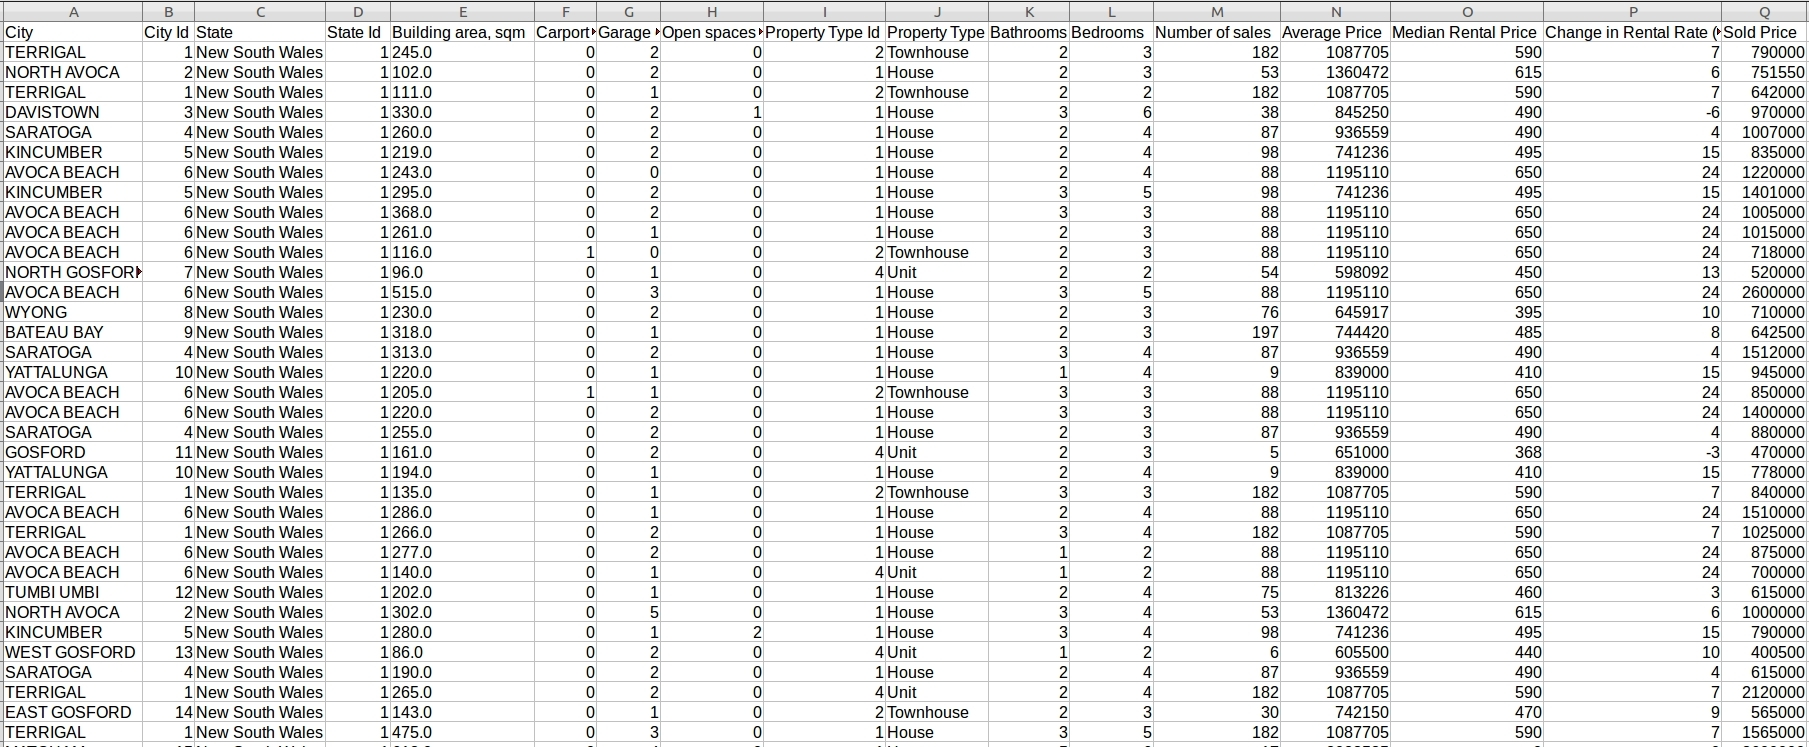
\includegraphics[scale=0.5]{csv.jpg}
    \caption{Исходные данные в csv формате}
    \label{fig:experiment:csv_example}
\end{sidewaysfigure}

Проведен анализ полученных данных. На рисунке~\ref{fig:experiment:hist_building_area} приведена гистограмма площадей
полученных объектов недвижимости, которая позволяет говорить что наиболее популярная недвижмиость имеет площадь от 100
до 150 квадратных метров.

\begin{figure}[!ht]
  \centering
  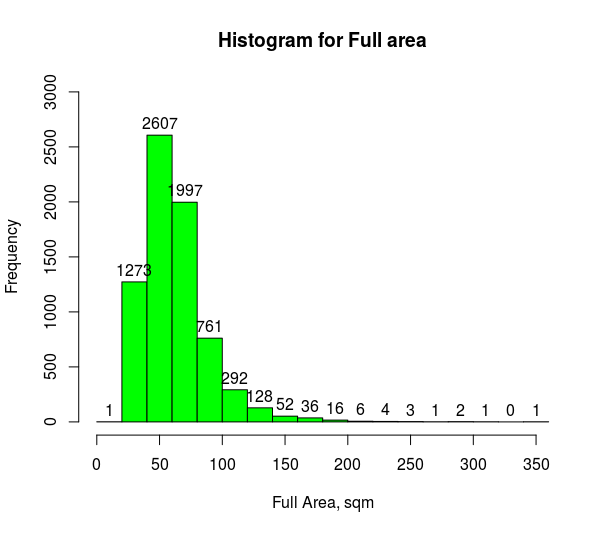
\includegraphics[scale=1]{hist_building_area.png} 
  \caption{Гистограмма площадей}
  \label{fig:experiment:hist_building_area}
\end{figure}

На рисунке~\ref{fig:experiment:barplot_bathrooms} приведена гистограмма душевых комнат
полученных объектов недвижимости, на которой видно что подавляющее большинство домов имеют 1 или 2 душевые комнаты.
\pagebreak

\begin{figure}[!ht]
  \centering
  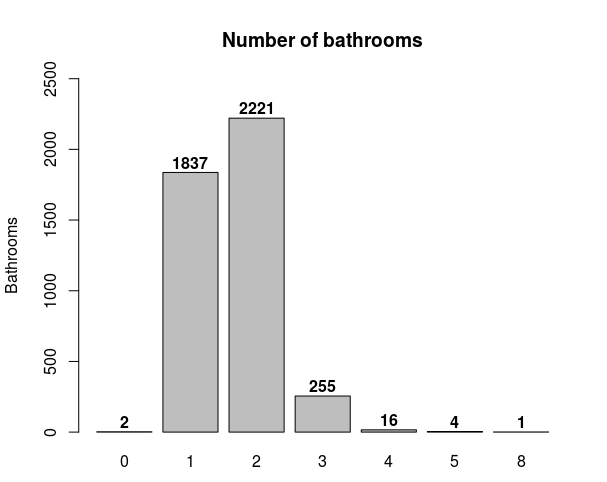
\includegraphics[scale=0.6]{barplot_bathrooms.png} 
  \caption{Гистограмма душевых комнат}
  \label{fig:experiment:barplot_bathrooms}
\end{figure}

На рисунке~\ref{fig:experiment:barplot_bedrooms} приведена гистограмма спален
полученных объектов недвижимости, на которой видно что большинство домов от двух до четырех спален.

\begin{figure}[!ht]
  \centering
  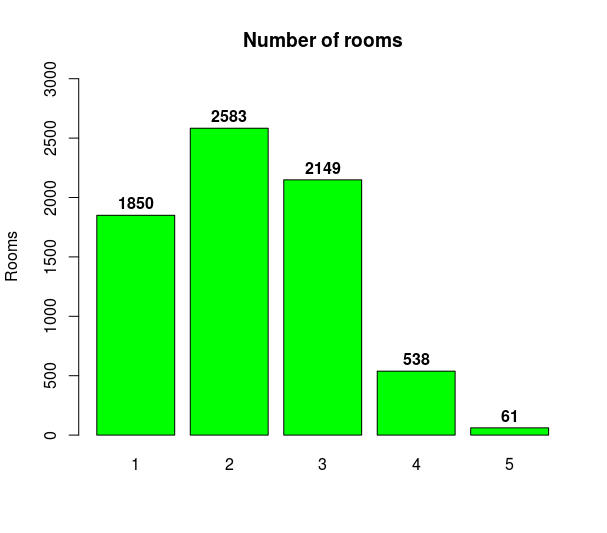
\includegraphics[scale=0.6]{barplot_bedrooms.png} 
  \caption{Гистограмма спален}
  \label{fig:experiment:barplot_bedrooms}
\end{figure}

На рисунке~\ref{fig:experiment:hist_sold_price} можно увидеть, что большинство квартир продаются в диапазоне
цен от 250 до 750 тысяч долларов.

\begin{figure}[!ht]
  \centering
  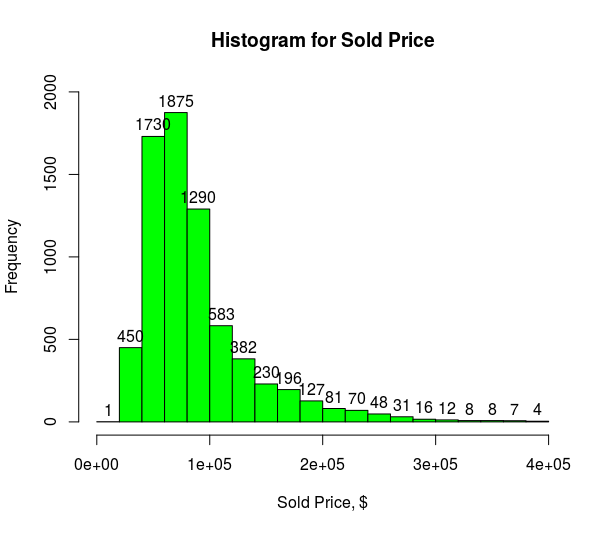
\includegraphics[scale=1]{hist_sold_price.png} 
  \caption{Гистограмма стоимости продажи}
  \label{fig:experiment:hist_sold_price}
\end{figure}
